
\subsection{闭合绘图（填充绘图下方的区域）}
\label{sec:pgfplots:closingplots}

\begin{command}{\closedcycle}
    在 |\addplot| 之后将 |\closedcycle| 作为 \meta{尾部路径命令} 使用，
    可从最后一个绘图坐标到第一个坐标绘制一条闭合线。

    当你希望填充绘图下方的区域时，请使用 |\closedcycle|。

\begin{codeexample}[]
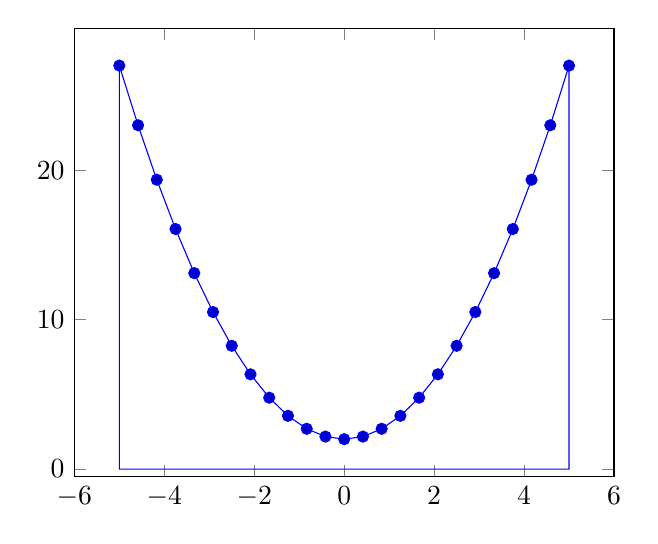
\begin{tikzpicture}
\begin{axis}
    \addplot {x^2+2} \closedcycle;
\end{axis}
\end{tikzpicture}
\end{codeexample}

\begin{codeexample}[]
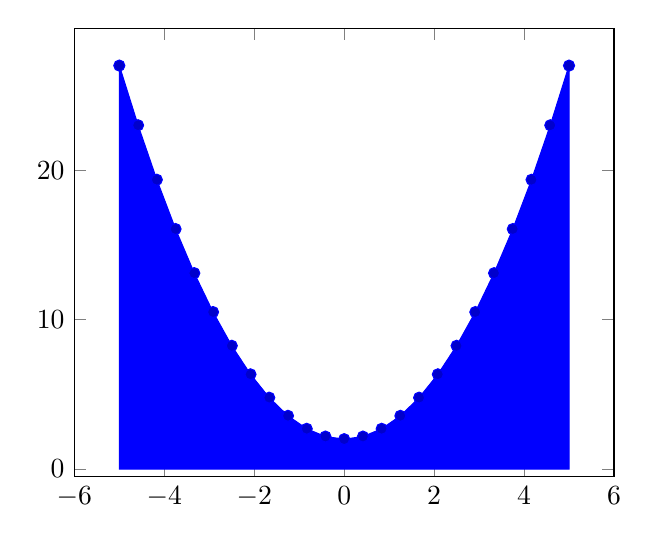
\begin{tikzpicture}
\begin{axis}
    \addplot+ [fill] {x^2+2} \closedcycle;
\end{axis}
\end{tikzpicture}
\end{codeexample}
    %
    对于堆叠图，|\closedcycle| 会将当前绘图与上一个绘图连接起来，
    而不是与 $x$ 轴连接。\footnote{堆叠图的实现需要一些额外的逻辑来
    确定填充区域：\lstinline{\\closedcycle} 会生成一个
    \texttt{plot coordinates} 命令，其中使用了上一个绘图的\emph{反向}
    坐标。这对最终用户通常无关紧要，但它假设绘图类型是对称的。
    由于阶梯图本质上是非对称的，\lstinline{\\closedcycle} 会将
    \texttt{const plot mark right} 用作 \texttt{const plot mark left}
    的反向序列。}
    %
\begin{codeexample}[]
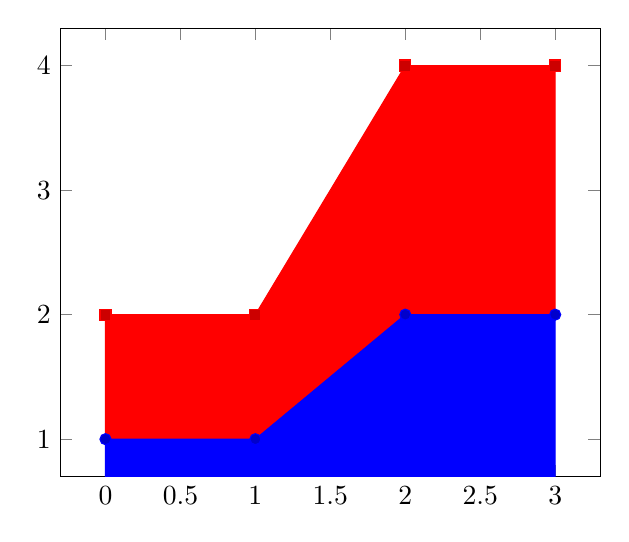
\begin{tikzpicture}
\begin{axis}[stack plots=y]
    \addplot+ [fill] coordinates {
        (0,1) (1,1) (2,2) (3,2)
    }
        \closedcycle
    ;
    \addplot+ [fill] coordinates {
        (0,1) (1,1) (2,2) (3,2)
    }
        \closedcycle
    ;
\end{axis}
\end{tikzpicture}
\end{codeexample}
\end{command}

闭合绘图同样适用于\emph{三维坐标轴}，详见第\pageref{sec:pgfplots:filled:line}页的\ref{sec:pgfplots:filled:line}节。

注意，|\closedcycle| 是为函数设计的（即每个 $x$ 至多对应一个 $y$
值的绘图）。对于任意曲线，你可以放心地使用 \tikzname{} 路径
\declareandlabel{--cycle}，它只是简单地连接最后一个路径元素和第一个：
%
\begin{codeexample}[]
\begin{tikzpicture}
\begin{axis}
    \addplot coordinates {
        (0,1) (1,2) (0,3) (-1,2)
    };
\end{axis}
\end{tikzpicture}
\end{codeexample}

\begin{codeexample}[]
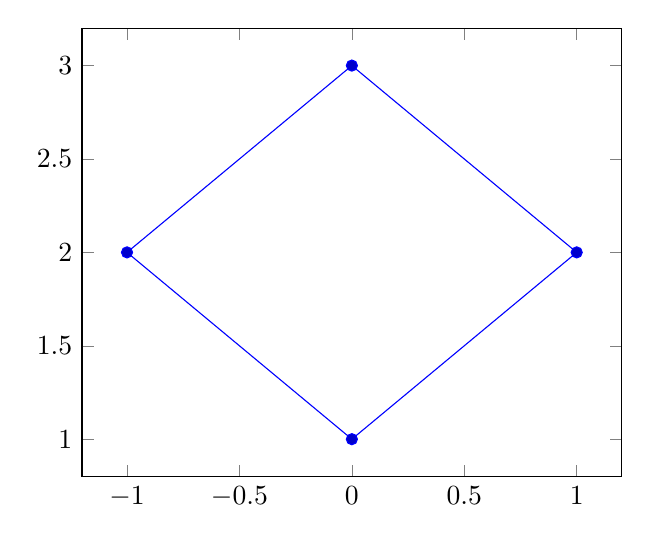
\begin{tikzpicture}
\begin{axis}
    \addplot coordinates {
        (0,1) (1,2) (0,3) (-1,2)
    }
        --cycle
    ;
\end{axis}
\end{tikzpicture}
\end{codeexample}

\begin{codeexample}[]
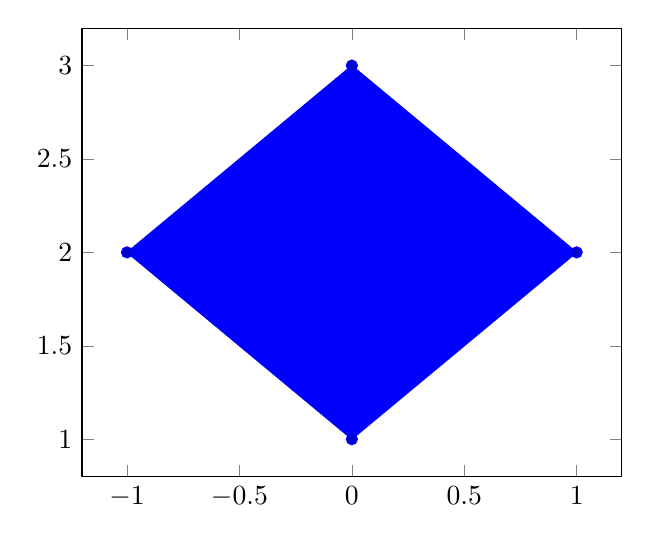
\begin{tikzpicture}
\begin{axis}
    \addplot+ [fill] coordinates {
        (0,1) (1,2) (0,3) (-1,2)
    }
        --cycle
    ;
\end{axis}
\end{tikzpicture}
\end{codeexample}

实际上，|--cycle| 是 \cite{tikz} 的一条路径指令；它连接一条路径的
第一个和最后一个坐标。注意，对于 |fill| 填充的路径，这一操作会自动完成。
